\chapter{Results} \label{ch:results}

Looking back at the analysis of the Gray-Scott system by Pearson, in particular \refFig{fig:fk_pspace}, the least stable regions of $F, k$ occur near the bifurcation lines\rf{pearson_1993}. We would expect that the most complex patterns with $F, k$ in this region would have higher entropy. Indeed, the results of the computation described in \refChapt{ch:methods} agree well with our expectations. The plot in \refFig{fig:fk_entropy} shows the entropy $S$ of the Gray-Scott system for chemical $V$ as $F, k$ is varied. Note that systems of higher $S$, given by the light regions of the plot, occur more densely near the dotted line which indicates Hopf bifurcation.

\begin{figure}[h]
	\centering
	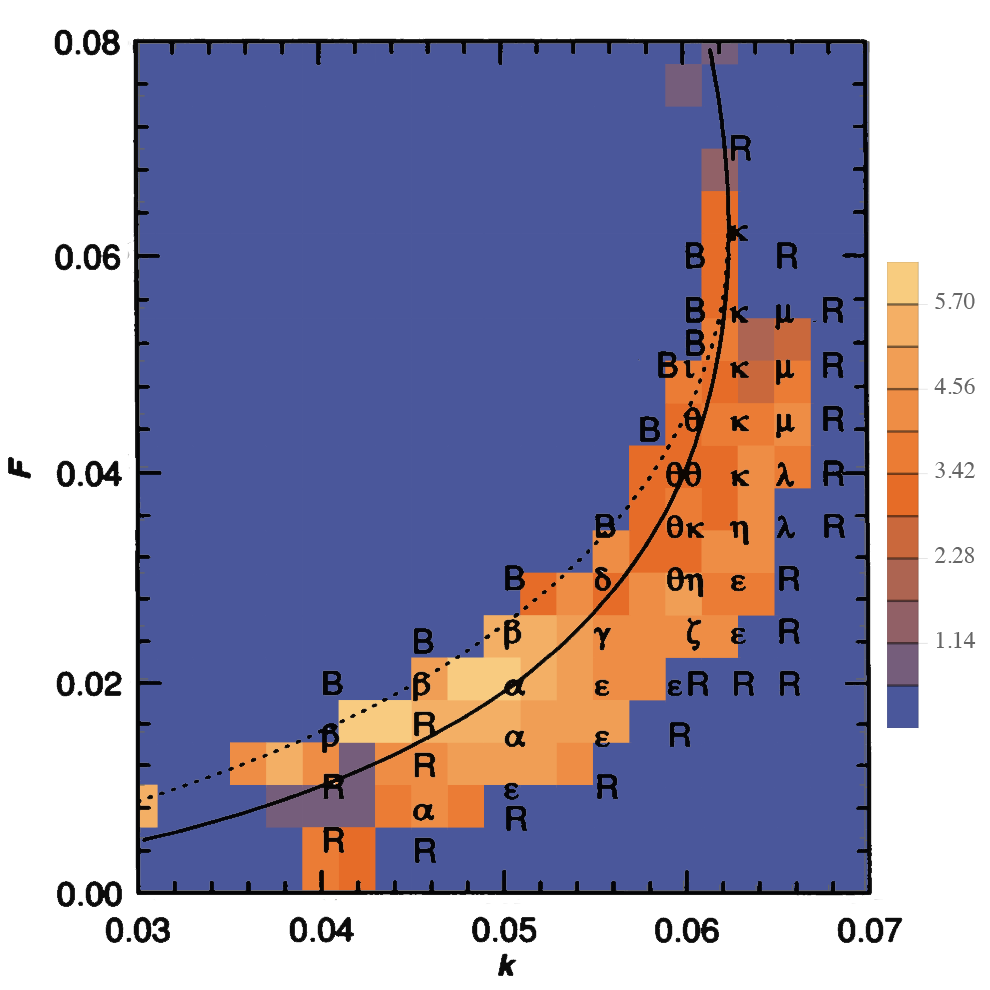
\includegraphics[width=0.8\textwidth]{fk_entropy.png}
	\caption{A heat-map style plot of entropy $S$ for the systems described by discrete values of $F, k$ for chemical $V$. The phase diagram as seen in \refFig{fig:fk_pspace} is shown on top of the map to illustrate its agreement with analysis by Pearson\rf{pearson_1993}.} \label{fig:fk_entropy}
\end{figure}